\begin{figure*}[t] 
\begin{center}
%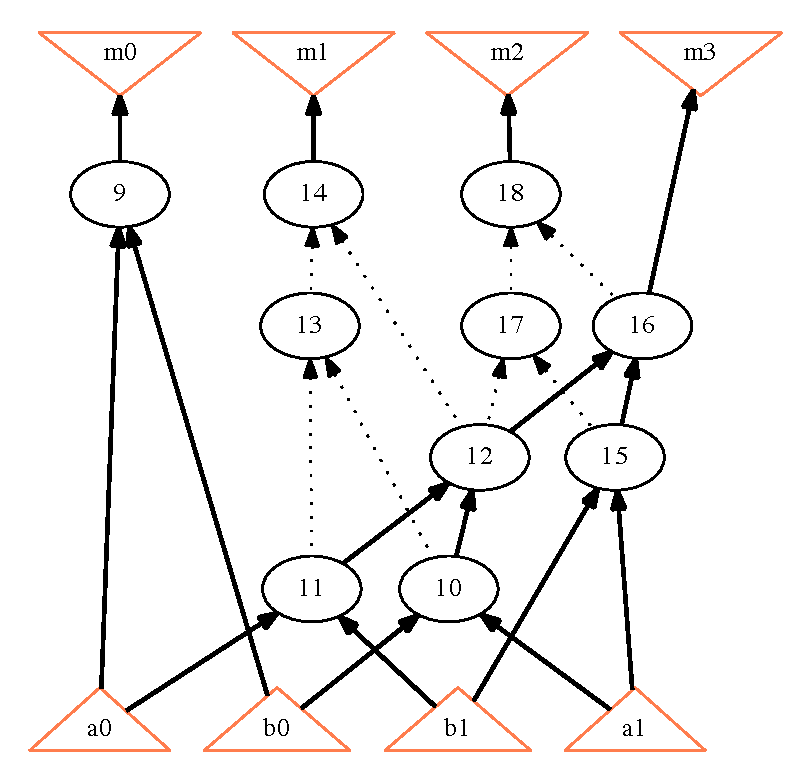
\includegraphics[scale=0.4]{../figs/2-bit-mult-aig.eps}
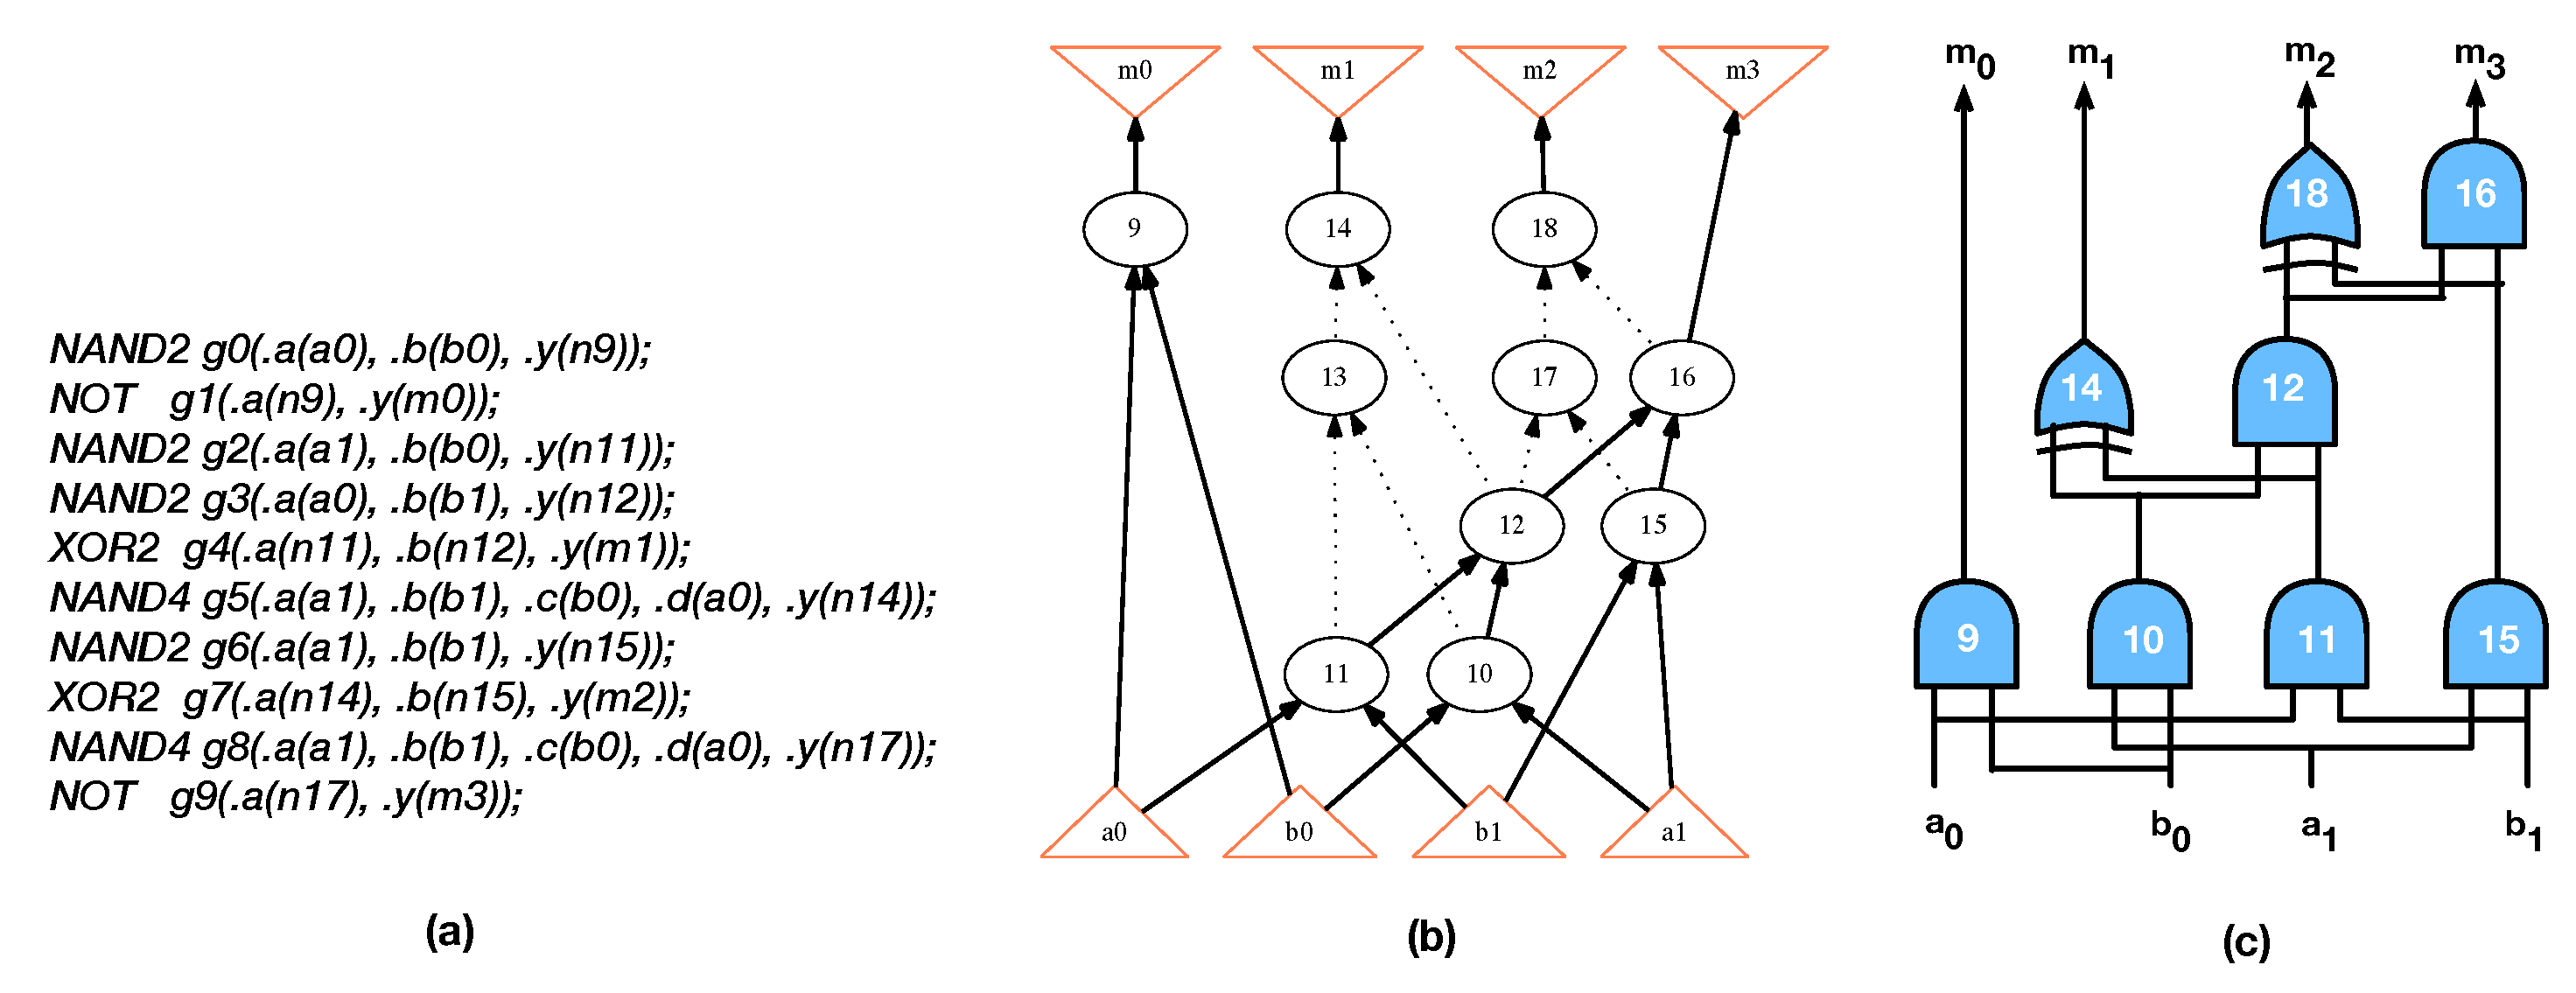
\includegraphics[scale=0.25]{../figs/aig-to-gatenetlist.eps}
\caption{\color{red}(a) Post-synthesized 2-bit multiplier gate-level netlist; (b) The AIG of the 2-bit multiplier shown in Figure \ref{fig:2-bit-mult-aig}(a); (c) Detected unobserved functions from the AIG and the correspondences to AIG nodes. The index value in Figure \ref{fig:2-bit-mult-aig}(c) corresponds to the hash value of each node in Figure \ref{fig:2-bit-mult-aig}(b). }
\vspace{-3mm}
\label{fig:2-bit-mult-aig}
\end{center}
\end{figure*}

\section{Approach} \label{sec:approach}

This section presents the algebraic rewriting approach based on AIGs. Similarly to \cite{ciesielski2015verification}, the algebraic rewriting process rewrites the output signature for all AIG nodes in a {\color{red}reverse topological order}. As discussed in {\color{red}Section \rom{2}-E}, the rewriting order that provides a large number of polynomial reductions, has significant impact on the rewriting performance. However, there are many {\color{red}reverse topological orders} available in an AIG, since many nodes can have the same topological depth. This approach detects a {\color{red}reverse topological order} for algebraic rewriting that provides the maximum polynomial reduction. This is achieved by detecting pairs of MAJ3 and XOR3 nodes using AIG-based \textit{cut enumeration}. 
%\begin{figure}[!htb] 
%\begin{center}
%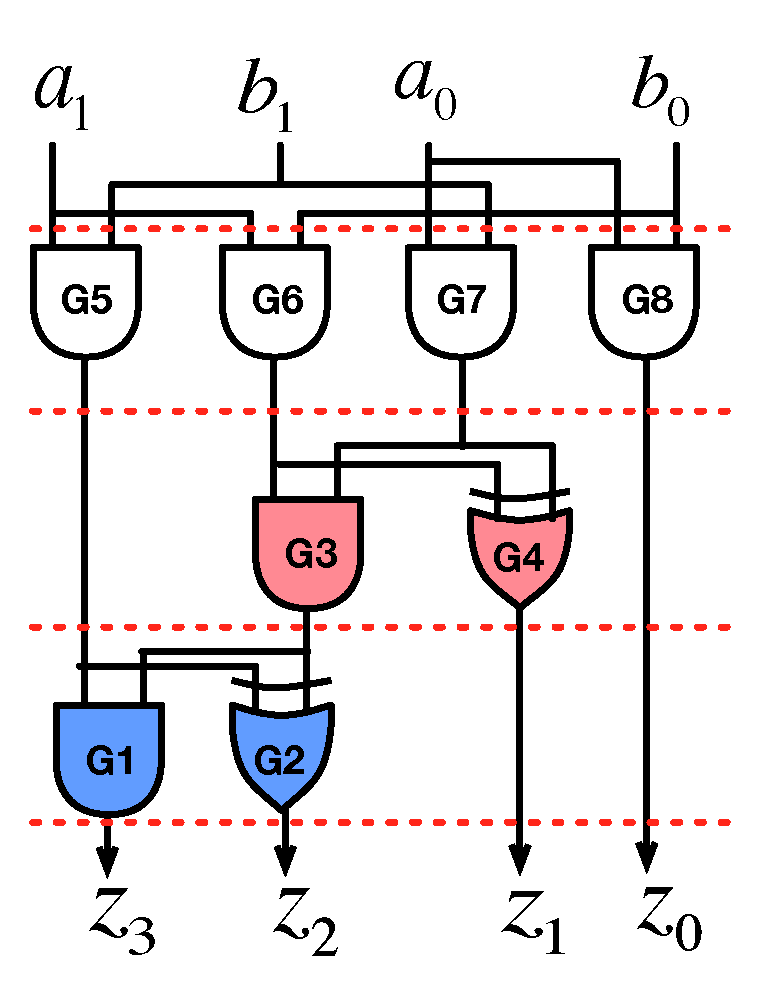
\includegraphics[scale=0.35]{../figs/order.eps}
%\caption{2-bit gate-level multiplier.}
%\label{fig:xor3-aig}
%\end{center}
%\end{figure}

\begin{algorithm}
\scriptsize
\caption{Algebraic Rewriting in AIG}\label{alg:algorithm}
\textbf{Input:} Gate-level netlist, output signature $Sig_{out}$  \\
\textbf{Output:} \textit{Pseudo-Boolean} expression extracted by rewriting 
\begin{algorithmic}[1]
\State Structural hashing the gate-level netlist into AIG, denoted \textit{G(V, E)}.
\State Detect all XOR3 and MAJ3 nodes in \textit{G(V, E)}.
\State Pair the XOR3 and MAJ3 if they have identical signals, denoted as $P$.
\State Topological sort \textit{G(V,E)} considering each element in $P$ as one node.
\State $i$ = 0; $F_{i}$ = $Sig_{out}$
\While{there are no elements remained in the {\color{red}reverse topological order}} %\Comment{We have the answer if r is 0}
\State Rewrite: $F_{i+1}$ = $F_{i}$ by substituting the variables with algebraic equations;
\State $i$ = i + 1
\EndWhile
\State \textbf{return} $F$ = $F_{i}$ (to be compared with $Sig_{in}$)
\end{algorithmic}
\end{algorithm}


\subsection{Outline of the Approach}

The proposed flow is outlined in Algorithm 1. The inputs to the algorithm are: the gate-level netlist and the output signature $Sig_{out}$. The flow includes three basic steps: 1) converting the gate-level implementation into AIG; 2) detecting all pairs of XOR3 and MAJ3 nodes with identical inputs; topological sorting the AIG nodes while considering the detected pairs as one element; and 3) applying algebraic rewriting from POs to PIs following the {\color{red}reverse topological order} determined in step 2). Note that XOR2 and MAJ2(AND2) are the special cases of XOR3 and MAJ3, where one of the inputs is constant zero. The second step is performed as follows: 

\begin{itemize}

\item Computing all 3-feasible (3-input) cuts of all AIG nodes.

\item Computing truth tables of all cuts.

\item Storing cuts in the hash table by their ordered set of inputs.

\item Detecting pairs of 3-input cuts with identical inputs belonging to different nodes, such that the Boolean functions of the two cuts with the shared inputs belong to the \textit{NPN} classes of XOR3 and MAJ3, respectively.

\end{itemize}

Note that, in this approach, matching the XOR3 and MAJ3 nodes does not require the inputs and outputs polarity to be the same. Instead, all the cut-points are matched without considering their complemented attributes. For example, instead of being an exact XOR3, the function of a 3-feasible cut can be either XOR3 or XNOR3. Similarly, instead of being exactly MAJ3, the function can be one of the eight functions forming the \textit{NPN} class of MAJ3 \cite{HuangWNM13}. To compute the cuts, the 3-input cut enumeration is performed in a {topological order} as described in \cite{PanL98}. The truth tables of the cuts are obtained as a by-product of the cut enumeration. Thus, when two fanin cuts are merged during the cut computation and the resulting cut is 3-feasible, the truth tables of fanin cuts are permuted to match the fanin order of the resulting cut. These truth tables are then ANDed or XORed, depending on the {\color{red}node function}, to get the resulting truth table. For the case of 3-input cuts, a dedicated pre-computation reduces the runtime of truth table computation to a small fraction of that of cut enumeration.

%Moreover, when detecting the pairs of XOR3 and MAJ3 nodes, the algebraic coefficient of MAJ3 node is not required to be 2$\times$ of the coefficient of the XOR3 node. Although the non-linear terms reductions between those XOR3 and MAJ3 happen only if the coefficients satisfy this condition, there are significant polynomial reductions provided by the detected XOR3 and MAJ3 pairs. This is based on an important observation that the XOR3 and MAJ3 with identical inputs, are likely to construct a one-bit addition (full-adder or half-adder). 

As soon as the XOR3 and MAJ3 pairs are detected, algebraic rewriting will be applied to the AIG network in a constrained {\color{red}reverse topological order}, in which each XOR3 and MAJ3 pair is considered as one element. This means that at one topological depth, whenever either XOR3 or MAJ3 node of a pair (or its complement) is rewritten, the subsequent rewritten node is of the other type. The AIG nodes with the same topological depth that do not belong to any pair are ordered in the decreasing order of their integer IDs. The algebraic rewriting ends when all elements in AIG network have been rewritten. The algorithm returns the extracted input signature. 


%\begin{figure}[t]
\scriptsize
\centering
\label{fig:2-bit-verilog}
\begin{tabular}{|l|}
\hline
\textit{\begin{tabular}[c]{@{}l@{}}and2 g0(.a(b0), .b(a0), .O(m0));\\ nand4 g1(.a(b1), .b(b0), .c(a1), .d(a0), .O(n10));\\ inv1 g2(.a(n10), .O(n11));\\ aoi22 g3(.a(b1), .b(a0), .c(b0), .d(a1), .O(n12));\\ nor2 g4(.a(n12), .b(n11), .O(m1));\\ and2 g5(.a(b1), .b(a1), .O(n14));\\ xnor2 g6(.a(n14), .b(n10), .O(m2));\\ nand4 g7(.a(b1), .b(b0), .c(a1), .d(a0), .O(n16));\\ inv1 g8(.a(n16), .O(m3));\end{tabular}} \\ \hline
\end{tabular}
\caption{Gate-level netlist of technology mapped 2-bit multiplier.}
\label{fig:2-bit-verilog}
\end{figure}





\textbf{Example 1 (2-bit CSA-multiplier):} The mapped gate-level netlist of a 2-bit CSA-multiplier is shown in Figure \ref{fig:2-bit-mult-aig}(a). First, the gate-level netlist is converted to an AIG representation, Figure \ref{fig:2-bit-mult-aig}(b). Then, a set of XOR3 nodes $X$, and a set of MAJ3 nodes $M$ are detected. $X$ = \{\textit{14, 18}\}, $M$ = \{12, 16\}. \textit{Node 14} is \textit{XOR3(10, 11, 0)} and \textit{node 12} is \textit{MAJ3(10, 11, 0)}, where \textit{nodes 10 and 11} and constant zero \textit{0} are the inputs; \textit{node 18} is \textit{XOR3(12, 15, 0)} and \textit{node 16} is \textit{MAJ3(12, 15, 0)}. Hence, two pairs of XOR3 and MAJ3 are generated, \textit{(14, 12)} and \textit{(18, 16)}. The order of rewriting is determined as follows: 1) \textit{node 18} is the node with highest depth; it is detected as a XOR3 and paired with a MAJ3 \textit{node 16}; hence, the first rewriting starts from node 18 and 16, and ends at node 12 and 15; 2) similarly to the first rewriting, the second rewriting starts from nodes 14 and 12, and ends at nodes 11 and 10; 3) the remaining AIG nodes are ordered by their index value in decreasing order. The logic network after detecting all XOR3 and MAJ3 functions are shown in Figure \ref{fig:2-bit-mult-aig}(c). %The largest size of the internal polynomial expression of our approach is XX. [compared to the old approach here.] 


\subsection{Detecting Redundant Polynomials}

Significant simplification of algebraic polynomial construction can be achieved not only by performing algebraic rewriting using a {\color{red}reverse topological order}, as discussed above, but also by detecting redundant polynomials, {\color{red}such as \textit{don't-care} polynomials and \textit{vanishing} polynomials \cite{sayedformal:date-2016}\cite{yu-isvlsi-16a}. Specifically, this section focuses on detecting \textit{don't-care polynomials} defined in \cite{yu-isvlsi-16a}, i.e., a set of polynomials that are included in the arithmetic function but excluded from the design.} %These polynomials are generated by observing that the signals removed to make design more efficient, contain algebraic information that is needed to cancel algebraic terms of the remaining output bits in the design. For example, the polynomial associated with the most significant bit (MSB) of an adder or a multiplier is such a polynomial. Such truncated designs are widely used in energy efficient applications by reducing critical paths and pruning the logic. However, automatically generating the redundant polynomials has not been addressed so far. 
%
{\color{red}These polynomials are identified by observing that in some designs, such as truncated multipliers, the removed signals contain algebraic information needed to cancel algebraic terms of the remaining output bits. Arithmetic operators are often truncated to reduce power consumption or speed up the critical path. Polynomial associated with the most significant bit (MSB) of an adder or a multiplier is an example of such a polynomial.}
Note that the logic obtained by removing such output bits is either a carry-out or a sum function of a full adder, implemented by MAJ3 and XOR3 functions. Hence, using the approach of detecting pairs of XOR3 and MAJ3 (Section \rom{3}-A), the XOR3/MAJ3 nodes that do not belong to any such pairs can also be identified. For example, in a $n$-bit CSA-multiplier with \textit{2n-1} output bits (with a MSB removed), MAJ3 with same inputs as an unpaired XOR3 is missing. Since one pair of XOR3 and MAJ3 is a full adder, removing the carry bit (and the MAJ3) makes the function an addition \textit{modulo 2}. In this case, the algebraic model of XOR3 (Equation 1) reduces to {\color{red}\textit{a + b + c - 2ab - 2ac - 2bc + 4abc mod 2}. In other words, the algebraic model of a $\oplus$ b $\oplus$ c in this case becomes \textit{a + b + c}}.
% This explains it for Reviewer 1: 
{\color{red}Specifically, the negation of the removed terms, \textit{-2ab - 2ac - 2bc + 4abc, gives the redundant polynomials detected for each unpaired XOR3}. 

%This is because MSBs of Booth multipliers are removed, i.e. the extra sign extension bits\footnote{A \textit{n}-bit Booth multiplier requires only \textit{2n} output bits. However, the Booth algorithm requires extra bits (sign extension) for intermediate computations. The number of extra bits added depends on the size of Booth encoding table.}. Those bits include a large number of algebraic monomials that can be used to reduce the size of internal polynomial during rewriting. In which case, they are considered as \textit{don't-care} polynomials. 

%To efficiently apply algebraic rewriting to the multipliers with output bits truncated, an approach that automatically generates \textit{don't-care} polynomials is presented. This approach is based on an observation that the logic obtained by removing output bits is either a carry-out function or a sum function of a 1-bit adder. It is known that MAJ3 and XOR3 are the components of a 1-bit adder. Hence, using the approach of detecting pairs of XOR3 and MAJ3 (Section \rom{3}-A), the XOR3/MAJ3 nodes that do not belong to any such pairs are also identified. For example, a $n$-bit CSA-multiplier with \textit{2n-1} output bits (with MSB removed), there is a missing MAJ3, i.e., the MAJ3s with identical inputs of an unpaired XOR3. Since one pair of XOR3 and MAJ3 is a 1-bit adder, removing the carry bit (MAJ3) makes the function to be {\color{red}\textit{a 1-bit addition mod 2}}. In this case, the algebraic model of XOR3 (Equation 1) is reduced to \textit{a $\oplus$ b $\oplus$ c = a+b+c mod 2}. %The negation of the removed terms by modulo 2, $- 2ac - 2bc + 4abc$, gives the redundant polynomials detected for each unpaired XOR3. 

\textbf{Example 2 (3-bit CSA-multiplier with MSB $z_{5}$ detected):} The AIG after detecting XOR3 and MAJ3 pairs of a 3-bit synthesized CSA-multiplier with MSB deleted is shown in Figure \ref{fig:3-bit-aig}. The detected XOR3 and MAJ3 pairs are represented using the ID of the root node of the XOR3 and MAJ3 nodes. We can see that there is one XOR3 (composed of two XOR2 nodes, \textit{41} and \textit{44}) with inputs $i_{36\_37}$, $i_{27\_29}$ and $i_{38}$, that cannot be paired with any MAJ3. This is simply because the synthesis process removed the redundant logic (last carry out) when the MSB has been removed. In this case, the algebraic model of that XOR3 reduces to $2^{4}z_{4}$($i_{49}$) = $2^4$($i_{36\_37}$ + $i_{27\_29}$ + $i_{38}$).



\begin{figure}[t] 
\begin{center}
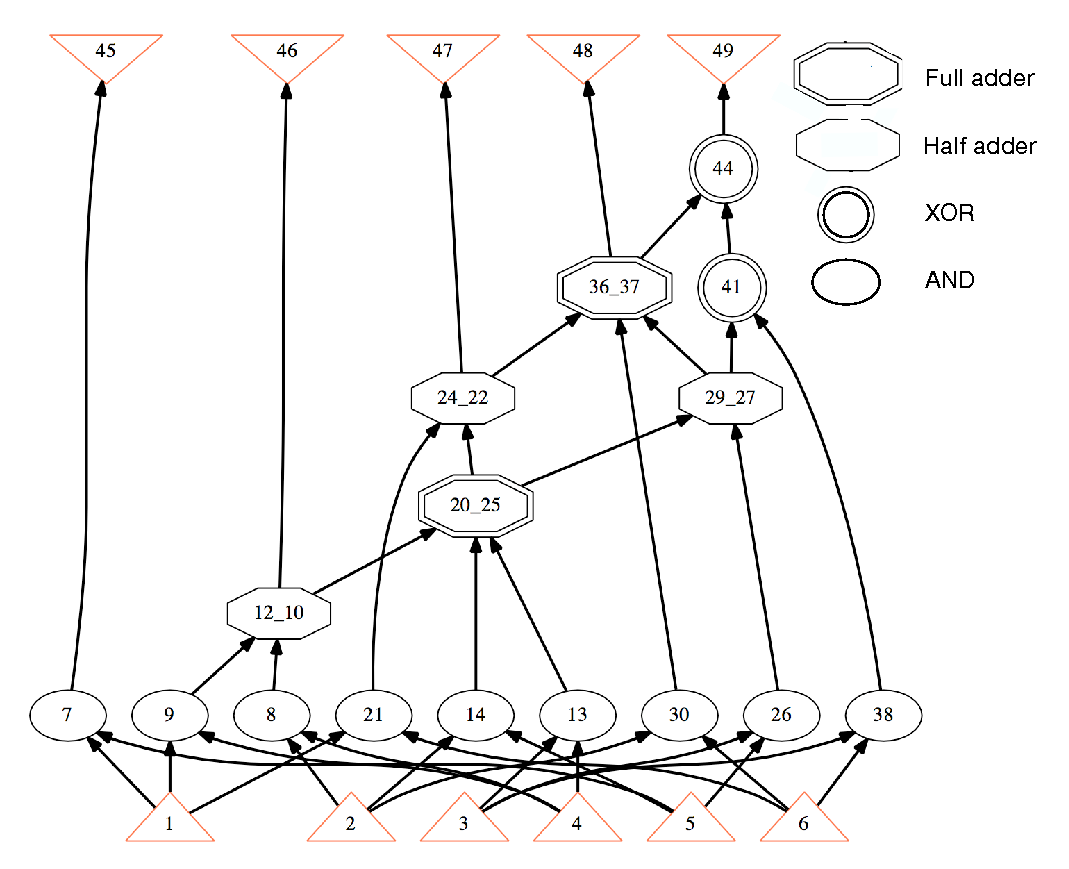
\includegraphics[scale=0.39]{../figs/truncate-mult3-new.eps}
\caption{\color{red}Detecting \textit{MAJ3-XOR3} of a 3-bit post-synthesized CSA-multiplier with MSB $z_{5}$ deleted.}
\vspace{-7mm}
\label{fig:3-bit-aig}
\end{center}
\end{figure}












